\documentclass[a4paper]{book}
% 设定页边距
\usepackage[top=1.1in,bottom=1.1in,left=1.25in,right=1in]{geometry}
% 引入graphicx的图形组件,dvips为图形加入引擎
\usepackage[dvips]{graphicx}
% 引入华丽页眉功能
\usepackage{fancyhdr}
% 引入并设定中文首行缩进功能
\usepackage{indentfirst}
\setlength{\parindent}{2em}
\setlength{\parskip}{0pt}
% 加载 CJK 相关宏包,并设置中文字体
\usepackage{CJKutf8, CJKnumb}
\newcommand{\song}{\CJKfamily{song}}
\newcommand{\hei}{\CJKfamily{hei}}
\newcommand{\kai}{\CJKfamily{kai}}
% 设定章节标题格式
\usepackage{titlesec}
\titleformat{\chapter}{\centering\LARGE\hei}{第\,\CJKnumber{\thechapter}\,章}{1em}{}
\titleformat{\section}{\large\hei}{\thesection}{1em}{}
\titleformat{\subsection}{\normalsize\hei}{\thesubsection}{1em}{}
% 设置页眉页脚
\usepackage{fancyhdr}
\pagestyle{fancy}
\renewcommand{\chaptermark}[ 1]{\markboth{\small 第\,\thechapter \,章\quad #1}{}}
\renewcommand{\sectionmark}[ 1]{\markright{\small\thesection \quad #1}{}}
\fancyhf{}
\fancyhead[ER]{ \leftmark}
\fancyhead[OL]{ \rightmark}
\fancyhead[EL,OR]{ $\cdot$\,\thepage\,$\cdot$ }
\renewcommand{\headrulewidth}{ 0.4pt}
\headheight=16pt
% 加入图形搜索路径
\graphicspath{{images/}}

\begin{document}
\begin{CJK}{UTF8}{song}
\title{GObject引用手册}
\author{TualatriX}
\date{\today}

\maketitle
\tableofcontents
\newpage

\chapter*{前言}

大多数现代的计算机语言都带有自己的类型和对象系统,并附带算法结构。正象GLib提供的基本类型和算法结构(如链表、哈希表等)一样,GObject的对象系统提供了一种灵活的、可扩展的、并容易映射(到其它语言)的面向对象的C语言框架。它的实质可以概括为:
\begin{itemize}
	\item 一个通用类型系统,用来注册任意的、轻便的、单根继承的、并能推导出任意深度的结构类型的界面,它照顾组合对象的定制、初始化和内存管理,类结构,保持对象的父子关系,处理这些类型的动态实现。也就是说,这些类型的实现是在运行时重置和卸载的。
	\item 一个基本类型的实现集,如整型,枚举型和结构型等。
	\item 一个基本对象体系之上的基本对象类型的实现的例子–GObject基本类型。
	\item 一个信号系统,允许用户非常灵活的自定义虚的或重载对象的方法,并且能充当非常有效力的通知机制。
	\item 一个可扩展的参数/变量体系,支持所有的能被用作处理对象属性或其它参数化类型的基本的类型。
\end{itemize}

\begin{CJK}{UTF8}{hei}
\chapter{背景}
\end{CJK}
GTK+和大多数GNOME库因为使用了GObject和比它更低一级的类型系统──GType,从而具有下面的特性:
\begin{itemize}
	\item 面向对象的基于C的API。
	\item 封装成其他编译型语言或动态解释语言的能力。
\end{itemize}
大多数程序员习惯于只使用编译型语言,或者只使用动态解析型语言,却不了解这些语言之间的关联。本文试图向你解释这些疑问,简洁地说明由GLib提供的解决办法。\footnote{即解决编译型语言与解释型语言的沟通问题。}

下面的章节将带你进入一个深层次的理解:关于GType和GObject是如何工作的,作为一个C开发者你将如何使用它们。
\begin{CJK}{UTF8}{hei}
\section{数据类型和编程}
\end{CJK}
关于程序语言的一种说法是:程序语言就是一种创建数据类型并使用函数去操作它们的语言。大多数语言提供了一系例基本类型和一些用于创建更复杂类型的原始类型。

在C语言中,它提供了一些基本类型如char, long, pointer等。在编译C代码的过程中,编译器将这些类型映射至编译器的目标机器的机器类型。如果你正在使用一个C解释器(虽然我从未看到过,不过理论上是有可能的),解释器(用于解释C代码并执行它的程序)在程序运行时,映射这些类型至目标机器的机器类型。

Perl和Python就是那种并不提供类似于C语言的类型的解释型语言。Perl和Python的开发者在操作变量时,变量的类型仅在第一次分配或在第一次使用时被强制为一个类型。解释器也提供一些自动转换的变量类型的方法。例如,在Perl中,一个具有整型值的变量可以在需要时被自动转换成字符串:


\begin{verbatim}
my $tmp = 10;
print "this is an integer converted to a string:" . $tmp . "\n";
\end{verbatim}

当然,在编码中同样允许明确使用一个由语言本身提供的类型转换句式。
\section{导出一个C的API}
C的API是常常是一些从二进制文件中导出的函数集和全局变量。C的函数可以有任意数量的参数和一个返回值。每个函数有唯一的由函数名确定的标识符,并且由C类型来描述参数和返回值。类似的,由API导出的全局变量也是由它们的名字和类型所标识。

一个C的API可能仅仅定义了一些类型集的关联。如果你了解函数调用和C类型至你所在平台的机器类型的映射关系,你可以在内存中解析到每个函数的名字从而找到这些代码所关联的函数的位置,并且构造出一个用在这个函数上的参数列表。最后,你可以用这个参数列表来呼叫这个目标C函数。

为了更好的讨论,请看下面这些C函数的例子和与其相关联在32位x86机器上由gcc产生的汇编代码:
\begin{verbatim}
static void function_foo (int foo)
{}
int main (int argc, char *argv[])
{
    function_foo (10);
    return 0;
}
push $0xa
call 0x80482f4 <function_foo>
\end{verbatim}
函数下显示的汇编代码是非常直观的: 第一个指令在堆栈上建立了十六进制的值0xa(十进制为10)作为一个32位的整型,并调用了function\_foo函数。就如你看到的,C函数的调用由gcc实现成了本地机器码的调用(这是实现起来最快的方法)。

现在,让我来告诉你,一个Python程序是如何调用这个C函数function\_foo的。为了完成调用,Python解释器需要做:

\begin{itemize}
	\item 找到函数所处的位置:这个意味着在C编译器编译成的二进制文件中寻找这个函数。
	\item 在可执行的内存中,载入有关这个函数的相关代码。
	\item 在调用这个函数前,将Python的参数转换为C兼容的参数。
	\item 用正确的方式调用这个函数。
	\item 将C函数的返回值转换成Python兼容的变量并将其返回至Python代码中。
\end{itemize}
上面所描述的处理过程是相当复杂的。不过有几个方法可以使它完全自动化,并且使得其过程对C和Python开发者而言都是透明的:
\begin{itemize}
	\item 第一个解决办法是手动编写一些“粘合代码”,当每个函数被导入或导出时,使用这些代码将Python的参数转换为C兼容的参数,并将C的返回值转换为 Python兼容的返回值。这个粘合代码将被连接到解释器上,从而解释器在解释Python程序时,可以完成程序中的调用C函数的工作。
	\item 另外一个更好的解决办法是自动产生粘合代码,当每个函数被导入或导出时,使用一个特殊的编译器来读取原始的函数签名。
	\item GLib用的解决办法是,使用GType库来保存在当前运行环境中的所有由开发者描述的对象的描述。这些“动态类型”库将被特殊的“通用粘合代码”来自动转换函数参数和进行函数调用在不同的运行环境之间。
\end{itemize}
这个由GType实现的解决方法有很大的优势,在运行环境边界之间的粘合代码只写一次就够了。下图或许会说明的更加清楚:

\begin{figure}[h]
\begin{center}
	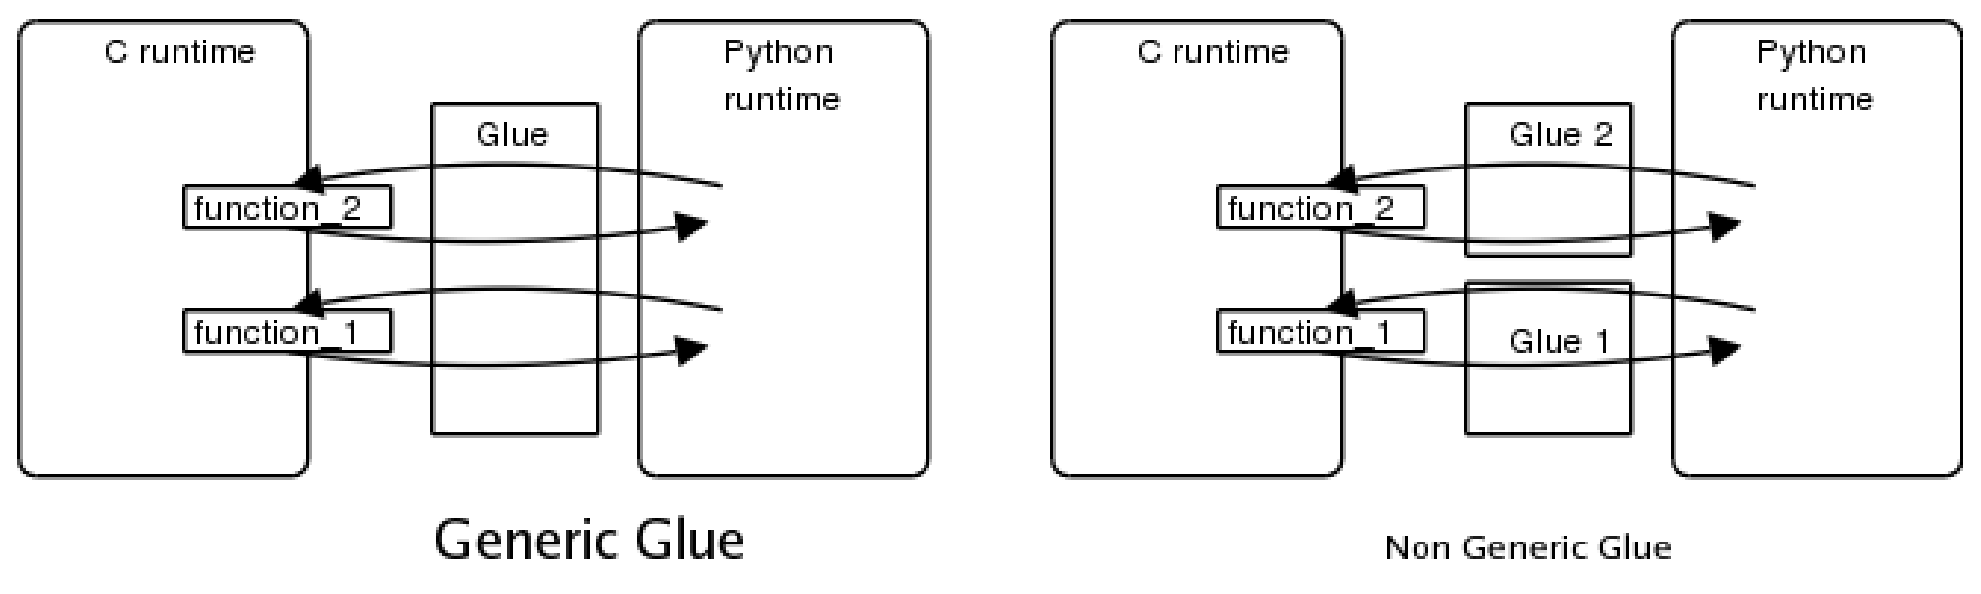
\includegraphics[width=1.0\textwidth]{glue}
	\caption{图}
\end{center}
\end{figure}

当前,至少存在于Python和Perl的通用粘合代码使得直接在Python或Perl使用用GType写的C对象成为可能,只要最少的工作量即可:没有必要去自动或手动去生成巨大的粘合代码。

这个目标被论证是值得称赞的,对它的追求影响了整个GType/GObject库。不过,C开发者很可能会被接下来几章所揭露的特性的复杂性所被难住,如果他们忘了GType/GObject库不仅仅是为了设计向C开发者提供面向对象的特性,也是为了透明的跨语言互通性。

\chapter{GLib动态类型系统}
由Glib类型系统操作的一个类型,比传统上所讲的Object类型更具一般化。下面查看类型系统中有关类结构和注册新类型的函数,是会对此最好的解释。

\begin{verbatim}
typedef struct _GTypeInfo               GTypeInfo;
struct _GTypeInfo
{
  /* interface types, classed types, instantiated types */
  guint16                class_size;

  GBaseInitFunc          base_init;
  GBaseFinalizeFunc      base_finalize;

  /* classed types, instantiated types */
  GClassInitFunc         class_init;
  GClassFinalizeFunc     class_finalize;
  gconstpointer          class_data;

  /* instantiated types */
  guint16                instance_size;
  guint16                n_preallocs;
  GInstanceInitFunc      instance_init;

  /* value handling */
  const GTypeValueTable *value_table;
};
GType g_type_register_static (GType             parent_type,
                              const gchar      *type_name,
                              const GTypeInfo  *info,
                              GTypeFlags        flags);
GType g_type_register_fundamental (GType                       type_id,
                                   const gchar                *type_name,
                                   const GTypeInfo            *info,
                                   const GTypeFundamentalInfo *finfo,
                                   GTypeFlags                  flags);
\end{verbatim}
\verb|g_type_register_static|和\verb|g_type_register_fundamental|这两个C函数定义在gtype.h中,并在gtype.c中具体实现。
你可以用来在程序的类型系统中注册一个新的GType。一般情况下你永远也不需要使用\verb|g_type_register_fundamental|(除非你是Tim Janik才会这样做),但是这次你要做,在最后一章会向你解释如何创建一个基本类型。

基本类型是不需要从任何其他类型取得的最顶级的类型, 相对的,其他非基本类型是继承于其他类型的。
在由\verb|g_type_init|初始化时,类型系统不仅仅初始化它的内部数据结构,同时也注册一些核心类型:其中一些是基本类型,其他则是从基本类型继承的。

不论是基本还是非基本类型,均由下面的定义步骤:
\begin{itemize}
	\item 类的大小:GTypeInfo的\verb|class_size|。
	\item 类的初始化函数(C++ 构造函数):GTypeInfo的\verb|base_init|和\verb|class_init|。
	\item 类的销毁函数(C++析构函数):GTypeInfo的\verb|base_finalize|和\verb|class_finalize|。
	\item 实例的大小(C++参数new):GTypeInfo中的\verb|instance_size|。
	\item 实例化策略(C++ 类的new operator):GTypeInfo的\verb|n_preallocs|。
	\item 复制函数(C++的复制操作):GTypeInfo的\verb|value_table|。
	\item 类的字符标志:GTypeFlags。
\end{itemize}
基本类型同样可以由GTypeFundamentalFlags来定义,并保存在GTypeFundamentallInfo中。非基本类型一般传递一个\verb|parent_type|至\verb|g_type_register_static|和\verb|g_type_register_dynamic|中,然后交给父类来定义。
\section{复制函数}
所有的glib类型(基本和非基本,类化和非类化,可实例化和不可实例化)的最大共同点是都可以通过单一的API来复制或指定它们。

GValue结构被用作所有类型的抽象的容器,它的极度简化的API(定义在gobject/gvalue.h)可以被使用请求\verb|value_table|函数被注册当类型注册中:举个例子,\verb|g_value_copy|复制了GValue的内容至另一个GValue。这与C++指派它的复制操作来修改默认的按位复制C++/C结构是类似的。

下面的代码向你展示了你是如何复制一个64位的整型,同样GObject的实例指针也是这样(代码在/gtype/test.c中):
\begin{verbatim}
static void test_int (void)
{
  GValue a_value = {0, };
  GValue b_value = {0, };
  guint64 a, b;

  a = 0xdeadbeaf;

  g_value_init (&a_value, G_TYPE_UINT64);
  g_value_set_uint64 (&a_value, a);

  g_value_init (&b_value, G_TYPE_UINT64);
  g_value_copy (&a_value, &b_value);

  b = g_value_get_uint64 (&b_value);

  if (a == b) {
    g_print ("Yay !! 10 lines of code to copy around a uint64.\n");
  } else {
    g_print ("Are you sure this is not a Z80 ?\n");
  }
}

static void test_object (void)
{
  GObject *obj;
  GValue obj_vala = {0, };
  GValue obj_valb = {0, };
  obj = g_object_new (MAMAN_BAR_TYPE, NULL);

  g_value_init (&obj_vala, MAMAN_BAR_TYPE);
  g_value_set_object (&obj_vala, obj);

  g_value_init (&obj_valb, G_TYPE_OBJECT);

  /* g_value_copy's semantics for G_TYPE_OBJECT types is to copy the reference.
     This function thus calls g_object_ref.
     It is interesting to note that the assignment works here because
     MAMAN_BAR_TYPE is a G_TYPE_OBJECT.
   */
  g_value_copy (&obj_vala, &obj_valb);

  g_object_unref (G_OBJECT (obj));
  g_object_unref (G_OBJECT (obj));
}
\end{verbatim}
上面代码的重点是关于复制指令的确切语义,并没有详细的定义复制是如何实现的。复制函数的实现可能是决定请求一新块的内存,并把数据从源复制到目的。或者可能是简单的增加实例的引用数和复制引用至新的GValue。

\verb|value_table|用于详细说明这些定义在gtype.h的函数的使用并彻底地描述在由GObject提供的API文档中,这是为什么我们不追究细节的原因。
\begin{verbatim}
typedef struct _GTypeValueTable         GTypeValueTable;
struct _GTypeValueTable
{
  void     (*value_init)         (GValue       *value);
  void     (*value_free)         (GValue       *value);
  void     (*value_copy)         (const GValue *src_value,
                                  GValue       *dest_value);
  /* varargs functionality (optional) */
  gpointer (*value_peek_pointer) (const GValue *value);
  gchar            *collect_format;
  gchar*   (*collect_value)      (GValue       *value,
                                  guint         n_collect_values,
                                  GTypeCValue  *collect_values,
                                  guint                collect_flags);
  gchar            *lcopy_format;
  gchar*   (*lcopy_value)        (const GValue *value,
                                  guint         n_collect_values,
                                  GTypeCValue  *collect_values,
                                  guint                collect_flags);
};
\end{verbatim}
有趣的是,你同样不需要详细指定一个\verb|value_table|在注册过程中,因为\verb|value_tables|一般从非基本类型的父类中继承,这意味着除非你想写一个基本类型,否则你将不需要提供一个新的\verb|value_table|因为它可以从父类继承\verb|value_table|。

请注意,另外一个注册函数是\verb|g_type_register_dynamic|。我们将不讨论这个函数,因为它与\_static版本非常相似。
\section{GLib的规范}
当用户在头文件中创建新类型时,有一些规范用户需要注意:
\begin{itemize}
	\item 使用\verb|object_method|的形式来定义函数名称:例如在一个bar类中定义一个名为foo的函数,则用\verb|bar_foo|。
	\item 使用前缀来避免与其他工程的命名空间冲突。如果你的库(或应用程序)名为Marman,那么所有的函数名称前缀为\verb|maman_|。举例:\verb|maman_object_method|。
	\item 创建一个宏命为\verb|PREFIX_OBJECT_TYPE|用来返回GType关联的对象类型。比如,Bar这个类在一个以maman前缀的库中,则使用\verb|MANMAN_BAR_TYPE|。另有一个不成文的规定是,定义一个使用全局静态变或一个名为\verb|prefix_object_get_type|的函数来实现这个宏。我们将在后面的章节中讨论这个函数。
	\item 创建一个宏命名为\verb|PREFIX_OBJECT(obj)|来返回一个指向PrefixObject类型的指针。这个宏用于必要时安全地强制转换一个静态类型。运行环境检查时,同样也是安全地执行动态类型。在处理过程中禁用动态类型检查是可行的。例如,我们可以创建\verb|MAMAN_BAR(obj)|来保持先前的例子。
	\item 如果类型是类化的,那么创建一个命令为\verb|PREFIX_OBJECT_CLASS(klass)|的宏。这个宏与前面那个是非常相似的:它以类结构的动态类型检查来进行静态转换,并返回一个指向PrefixObjectClass这个类型的类结构的指针。同样,例子为:\verb|MAMAN_BAR_CLASS|。
	\item 创建一个宏命名为\verb|PREFIX_IS_BAR (obj)|:这个宏用于判断输入的对象实例是否是BAR类型的。
	\item 如果类型是类化的,创建一个名为\verb|PREFIX_IS_OBJECT_CLASS (klass)|的宏,与上面的类似,返回输入的类型指针是否是OBJECT类型。
	\item 如果类型是类化的,创建一个名为\verb|PREFIX_OBJECT_GET_CLASS|,返回一个实例所属的类的类型指针。这个宏因为安全的原因,被静态和动态类型所使用,就像上面的转换宏一样。
\end{itemize}
至于这些宏的实现是非常直观的:一些数量的简单使用的宏由gtype.h提供。针对上面我们兴趣的例子,我们写了下面的代码来声明这些宏:
\begin{verbatim}
#define MAMAN_BAR_TYPE                  (maman_bar_get_type ())
#define MAMAN_BAR(obj)                  (G_TYPE_CHECK_INSTANCE_CAST ((obj), MAMAN_BAR_TYPE, MamanBar))
#define MAMAN_BAR_CLASS(klass)          (G_TYPE_CHECK_CLASS_CAST ((klass), MAMAN_BAR_TYPE, MamanBarClass))
#define MAMAN_IS_BAR(obj)          (G_TYPE_CHECK_INSTANCE_TYPE ((obj), MAMAN_BAR_TYPE))
#define MAMAN_IS_BAR_CLASS(klass) (G_TYPE_CHECK_CLASS_TYPE ((klass), MAMAN_BAR_TYPE))
#define MAMAN_BAR_GET_CLASS(obj)  (G_TYPE_INSTANCE_GET_CLASS ((obj), MAMAN_BAR_TYPE, MamanBarClass))
\end{verbatim}
下面的代码实现了\verb|maman_bar_get_type|这个函数:
\begin{verbatim}
GType maman_bar_get_type (void)
{
  static GType type = 0;
  if (type == 0) {
    static const GTypeInfo info = {
      /* You fill this structure. */
    };
    type = g_type_register_static (G_TYPE_OBJECT,
                                   "MamanBarType",
                                   &info, 0);
  }
  return type;
}
\end{verbatim}
\section{不可实例和不可类化的类型:基础类型}
在类型系统中,许多类型是不可实例化而且没有父类的。大多数这些类型是最基础的基本类型,如gchar,它由\verb|g_value_types_init|注册(在gvaluetypes.c中)。

如果想在类型系统中注册这样一个类型,你仅仅需要用0来填充GTypeInfo结构。
\begin{verbatim}
  GTypeInfo info = {
    0,                                /* class_size */
    NULL,                        /* base_init */
    NULL,                        /* base_destroy */
    NULL,                        /* class_init */
    NULL,                        /* class_destroy */
    NULL,                        /* class_data */
    0,                                /* instance_size */
    0,                                /* n_preallocs */
    NULL,                        /* instance_init */
    NULL,                        /* value_table */
  };
  static const GTypeValueTable value_table = {
    value_init_long0,                /* value_init */
    NULL,                        /* value_free */
    value_copy_long0,                /* value_copy */
    NULL,                        /* value_peek_pointer */
    "i",                        /* collect_format */
    value_collect_int,        /* collect_value */
    "p",                        /* lcopy_format */
    value_lcopy_char,                /* lcopy_value */
  };
  info.value_table = &value_table;
  type = g_type_register_fundamental (G_TYPE_CHAR, "gchar", &info, &finfo, 0);
\end{verbatim}

使用不可实例的类型似乎是无用的:定义一个不能实例化的类型有什么好处呢?大多数这种类型与GValue用作一块:一个GValue由一个整型或一个字符串来初始化,再被传递了一个已注册类型的\verb|value_table|。GValue(以基本类型延伸)最有用的时候是在与对象的属性和信号用在一块时。
\section{可实例化的类型:对象}
一个以类来注册,并声明为可实例化的类型常常称作对象。GObject(定义在The GObject base class中)是最有名的一个可实例化的类了,其他相似的类都继承于这个基本类来进行开发,他们都基于下面所述的基本特征。

下面的例子告诉你怎样才可以在类型系统中注册这样一个基本的类。
\begin{verbatim}
typedef struct {
  GObject parent;
  /* instance members */
  int field_a;
} MamanBar;

typedef struct {
  GObjectClass parent;
  /* class members */
  void (*do_action_public_virtual) (MamanBar *self, guint8 i);

  void (*do_action_public_pure_virtual) (MamanBar *self, guint8 i);
} MamanBarClass;

#define MAMAN_BAR_TYPE (maman_bar_get_type ())

GType 
maman_bar_get_type (void)
{
  static GType type = 0;
  if (type == 0) {
    static const GTypeInfo info = {
      sizeof (MamanBarClass),
      NULL,           /* base_init */
      NULL,           /* base_finalize */
      (GClassInitFunc) foo_class_init,
      NULL,           /* class_finalize */
      NULL,           /* class_data */
      sizeof (MamanBar),
      0,              /* n_preallocs */
      (GInstanceInitFunc) NULL /* instance_init */
    };
    type = g_type_register_static (G_TYPE_OBJECT,
                                   "BarType",
                                   &info, 0);
  }
  return type;
}
\end{verbatim}
在调用\verb|maman_bar_get_type|之前,名为BarType的继承于\verb|G_TYPE_OBJECT|的类将在类型系统中被注册。

每个对象必须定义为两个结构:它的类结构和它的实例结构。所有的类结构的第一个成员必须是一个GTypeClass结构。所有的实例结构的第一个成员必须是GTypeInstance结构。下面显示了这些来自gtype.h的C类型的声明:

\begin{verbatim}
struct _GTypeClass
{
  GType g_type;
};
struct _GTypeInstance
{
  GTypeClass *g_class;
};
\end{verbatim}
这些约束使得类型系统可以确保每个对象的实例(由指向该对象的实例结构的指针所标识) 的首字节指向该对象的类结构。

这个关系可以由下面的例子来很好的解释:让我们来看看这个继承于对象A的对象B。

\begin{verbatim}
/* A definitions */
typedef struct {
  GTypeInstance parent;
  int field_a;
  int field_b;
} A;
typedef struct {
  GTypeClass parent_class;
  void (*method_a) (void);
  void (*method_b) (void);
} AClass;

/* B definitions. */
typedef struct {
  A parent;
  int field_c;
  int field_d;
} B;
typedef struct {
  AClass parent_class;
  void (*method_c) (void);
  void (*method_d) (void);
} BClass;
\end{verbatim}
上述标准的C结构定义指示了这个C结构的第一个领域存储着类的结构。This means that the first field of an instance of an object B is A’s first field which in turn is GTypeInstance’s first field which in turn is \verb|g_class|, a pointer to B’s class structure.

多亏了这些简单的条件,所以按下面的方法来就可能取得每个对象实例的类型:
\begin{verbatim}
B *b;
b->parent.parent.g_class->g_type
\end{verbatim}
或者,更快的:
\begin{verbatim}
B *b;
((GTypeInstance*)b)->g_class->g_type
\end{verbatim}
\subsection{初始化和销毁}
实例化这些类型可以用\verb|g_type_create_instance|来完成:
\begin{verbatim}
GTypeInstance* g_type_create_instance (GType          type);
void           g_type_free_instance   (GTypeInstance *instance);
\end{verbatim}

\verb|g_type_create_instance|将查找请求的类型所关联的类型信息结构。然后由用户声明的实例的大小和实例化策略(如果\verb|n_preallocs|设置为一个非零值,类型系统将会把对象的实例结构分配在内存块上,而不将依次分配每个实例)将得到一个缓存来保存对象实例的结构。

如果实例是这个对象第一次创建的,那么类型系统必须创建一个类结构:它为其分配一个缓冲来保存这个对象的类结构并初始化它。它先用父类的类结构覆盖(如果没有父类,它将初始化为零),然后从最顶层的基本对象至最底层的对象调用\verb|base_class_initialization|函数(GBaseInitFunc)。对象的类初始化函数(GClassInitFunc)被调用来完成类结构的初始化。最终,这个类的接口被初始化了(我们将在后面讨论接口初始化)。

一旦类型系统有一个指向初始化的类结构的指针,它设置对象的实例类指针指向对象的类结构并调用实例的初始化函数(GInstanceInitFunc),同样是从顶到底的顺序。

对象的实例的销毁非常简单,通过\verb|g_type_free_instance|即可:实例结构被返回到实例池中,如果这是对象的还有一个而且是最后一个存活的实例,那么这个类即被摧毁。

类的销毁(关于这个销毁的另一概念是GType的终结)的过程与初始化的刚好对称:接口先被销毁。然后,调用类终结函数\verb|class_finalize|(ClassFinalizeFunc)。最终,将\verb|base_class_finalize|(GBaseFinalizeFunc)从底至顶的调用,直到类结构被销毁。

很多读者已经明白了,基本的初始化/终结化过程与C++的构造/析构函数非常相似。实际上细节是非常不同的,千万不要被表现的相似所迷惑。特别是,大多数用户开始认识到GType中并不存在类似于C++的构造器(这实际上是一个方法列表,由对象实例来调用所有有继承关系的方法),它必须建立在由 GType提供的特定的设施里。同样的,GType没有实例销毁机制。这是用户的职责,在现存的GType代码的顶端来实现正确的销毁(这就是 GObject做的事情)。

举个例子,如果从A继承的对象B被实例化了,GType将只调用对象B的\verb|instance_init|回调函数,而C++运行环境将先调用对象A的构造器,接着再是对象B。事实上,C++代码与GType的\verb|base_init|和\verb|class_init|回调是等同的,不过C++常常是不需要这些的,因为它并不能真的在运行时创建类型。

关于实例化和终结化的处理过程可以归纳如下:

\section{不可实例的类型:接口}
GType的接口(Interface)与Java的接口非常类似。它允许描述一个通用的API,使得多个类可以粘合在一起。想像一下,Hi-Fi音响设备中的暂停和播放按钮──这可以被视做一个回放接口。如果你知道你要做什么,你可以用来这个接口来控制你的CD机,MP3或其他使用相同符号的东西。要声明一个接口,你需要注册一个从GTypeInterface继承的不可实例的类型。下面的代码声明了这样的一个接口:

\begin{verbatim}
#define MAMAN_IBAZ_TYPE                (maman_ibaz_get_type ())
#define MAMAN_IBAZ(obj)                (G_TYPE_CHECK_INSTANCE_CAST ((obj), MAMAN_IBAZ_TYPE, MamanIbaz))
#define MAMAN_IS_IBAZ(obj)             (G_TYPE_CHECK_INSTANCE_TYPE ((obj), MAMAN_IBAZ_TYPE))
#define MAMAN_IBAZ_GET_INTERFACE(inst) (G_TYPE_INSTANCE_GET_INTERFACE ((inst), MAMAN_IBAZ_TYPE, MamanIbazInterface))

typedef struct _MamanIbaz MamanIbaz; /* dummy object */
typedef struct _MamanIbazInterface MamanIbazInterface;

struct _MamanIbazInterface {
  GTypeInterface parent;

  void (*do_action) (MamanIbaz *self);
};

GType maman_ibaz_get_type (void);

void maman_ibaz_do_action (MamanIbaz *self);
\end{verbatim}

这里用非常简单的方法来实现\verb|maman_ibaz_do_action|这个接口函数:
\begin{verbatim}
void maman_ibaz_do_action (MamanIbaz *self)
{
  MAMAN_IBAZ_GET_INTERFACE (self)->do_action (self);
}
\end{verbatim}

\verb|maman_ibaz_get_type|注册了一个从\verb|G_TYPE_INTERFACE|继承的名为MamanIBaz的类型。在继承树中,所有的接口必须是\verb|G_TYPE_INTERFACE|的子类。

一个接口只有一个包含GTypeInterface的结构来定义。接口的结构应该要包含一个函数指针指向这个接口的方法。用类似于\verb|maman_ibaz_do_action|的方法在每个接口方法中定义帮助函数,可以使得我们直接调用接口方法,这是一个良好的风格。

一旦一个接口的类型被注册后,你必须来实现这个接口。其中,命名为\verb|maman_baz_get_type|注册一个名为MamanBaz的由GObject继承来的新的GType,并在接口Interface中实现。
\begin{verbatim}
static void maman_baz_do_action (MamanIbaz *self)
{
  g_print ("Baz implementation of IBaz interface Action.\n");
}


static void
baz_interface_init (gpointer         g_iface,
                    gpointer         iface_data)
{
  MamanIbazInterface *iface = (MamanIbazInterface *)g_iface;
  iface->do_action = maman_baz_do_action;
}

GType 
maman_baz_get_type (void)
{
  static GType type = 0;
  if (type == 0) {
    static const GTypeInfo info = {
      sizeof (MamanBazInterface),
      NULL,   /* base_init */
      NULL,   /* base_finalize */
      NULL,   /* class_init */
      NULL,   /* class_finalize */
      NULL,   /* class_data */
      sizeof (MamanBaz),
      0,      /* n_preallocs */
      NULL    /* instance_init */
    };
    static const GInterfaceInfo ibaz_info = {
      (GInterfaceInitFunc) baz_interface_init,    /* interface_init */
      NULL,               /* interface_finalize */
      NULL          /* interface_data */
    };
    type = g_type_register_static (G_TYPE_OBJECT,
                                   "MamanBazType",
                                   &info, 0);
    g_type_add_interface_static (type,
                                 MAMAN_IBAZ_TYPE,
                                 &ibaz_info);
  }
  return type;
}
\end{verbatim}
\verb|g_type_add_interface_static|记录了在类型系统中如FooInterface来实现的接口(\verb|foo_interface_get_type|返回FooInterface的类型),GInterfaceInfo保存着关于接口实现的信息:
\begin{verbatim}
struct _GInterfaceInfo
{
  GInterfaceInitFunc     interface_init;
  GInterfaceFinalizeFunc interface_finalize;
  gpointer               interface_data;
};
\end{verbatim}

\subsection{接口初始化}
当一个对象的第一次注册一个接口实现时, 它的类结构由下述的方法所初始化。等类结构初始化后,函数\verb|type_class_init_Wm|(实现在gtype.c)会初始化由类关联的每个接口,以\verb|type_iface_vtable_init_Wm|调用每个接口。

首先为接口结构分配内存缓冲,父接口结构先被复制(父接口先被初始化)。如果没有父接口,接口结构将由0初始化。\verb|g_type|和\verb|g_instance_type|将在其后被初始化:\verb|g_type|被设置为最先起源的接口,\verb|g_instance_type|被设置为最先起源的实现这个接口的类。

最终,接口的最顶层的\verb|base_init|函数和实现接口的\verb|interface_init|被调用。了解下面是重要的:如果有一个接口有多个\verb|base_init|和\verb|interface_init|的实现,那么每个实现都被调用一次以初始化。

\verb|base_init|函数保持了一个本地静态变量用来确保这个接口类型只被初始化一次而不管它是否被实现了几次:
\begin{verbatim}
static void
maman_ibaz_base_init (gpointer g_iface)
{
  static gboolean initialized = FALSE;

  if (!initialized) {
    /* create interface signals here. */
    initialized = TRUE;
  }
}
\end{verbatim}
如果你发现接口很烦,确实如此。它确实很烦,但是我也没办法啊。我只有把接口的过程归纳一下了!

\subsection{接口的销毁}

当最后一个实现某接口的实例被销毁以后,这个与类型相关联的接口实现也将由\verb|type_iface_vtable_finalize_Wm|来销毁(gtype.c)

\verb|type_iface_vtable_finalize_Wm|调用了第一个实现的\verb|interface_finalize|函数,接着是接口最底层的\verb|base_finalize|函数。

同样,下面的理解非常重要,如“接口的初始化”中描述的,\verb|interface_finalize|和\verb|base_finalize|都将被调用来确保一个接口的实现被正确的销毁。例如,如果你曾用过其中一个函数,你将需要使用一个静态的整形来保持有关实例实现的接口的数量,这样接口的类才会只被销毁一次(当整型变量为0时)。

上面的处理过程总结如下:

你已经读完了这章,现在你可以忘记它了。请尽可能快地忘记它!

\chapter{基类:GObject}
前面两个章节讨论了Glib动态类型系统的细节和它的信号控制系统。GObject库同时也包括了一个最基本的类型即基类,即为GObject。

GObject是一个类化的可实例的基类。它实现了:
\begin{itemize}
	\item 使用引用计数的内存管理。
	\item 实例的构造和析构 。
	\item 使用set/get函数对进行的一般性属性操作。
	\item 简易使用的信号机制。
\end{itemize}
所有使用GLib类型系统的GNOME库(如GTK+和GStreamer)都由GObject继承,所以了解有关它是如何工作的细节是如此重要。

\section{对象实例}
\verb|g_object_new|系列函数可以被用作实例化由GObject基本类型继承的一些GType。所有的这些函数确保类和实例的结构被Glib的类型系统正确的初始化,然后调用一个或别的构造类方法用于:

\begin{itemize}
	\item 通过\verb|g_type_create_instance|来分配和清理内存。
	\item 初始化对象的实例用构造属性。
\end{itemize}

尽管你可以期待所有的类和实例成员(指向父类的部分)都会设置为0,但是尽量考虑自己明确地去设置它们。

由GObject继承的对象们允许重载它的类构造方法:在做下面之前它们需要连接到父类的构造方法:
\begin{verbatim}
  GObject*   (*constructor)     (GType                  type,
                                 guint                  n_construct_properties,
                                 GObjectConstructParam *construct_properties);
\end{verbatim}

下面的代码显示MamanBar重载了父类的构造器:

\begin{verbatim}
#define MAMAN_TYPE_BAR                  (maman_bar_get_type ())
#define MAMAN_BAR(obj)                  (G_TYPE_CHECK_INSTANCE_CAST ((obj), MAMAN_TYPE_BAR, MamanBar))
#define MAMAN_BAR_CLASS(klass)          (G_TYPE_CHECK_CLASS_CAST ((klass), MAMAN_TYPE_BAR, MamanBarClass))
#define MAMAN_IS_BAR(obj)          (G_TYPE_CHECK_INSTANCE_TYPE ((obj), MAMAN_TYPE_BAR))
#define MAMAN_IS_BAR_CLASS(klass) (G_TYPE_CHECK_CLASS_TYPE ((klass), MAMAN_TYPE_BAR))
#define MAMAN_BAR_GET_CLASS(obj)  (G_TYPE_INSTANCE_GET_CLASS ((obj), MAMAN_TYPE_BAR, MamanBarClass))

typedef struct _MamanBar MamanBar;
typedef struct _MamanBarClass MamanBarClass;

struct _MamanBar {
  GObject parent;
  /* instance members */
};

struct _MamanBarClass {
  GObjectClass parent;

  /* class members */
};

/* used by MAMAN_TYPE_BAR */
GType maman_bar_get_type (void);

static GObject *
maman_bar_constructor (GType                  type,
                       guint                  n_construct_properties,
                       GObjectConstructParam *construct_properties)
{
  GObject *obj;

  {
    /* Invoke parent constructor. */
    MamanBarClass *klass;
    GObjectClass *parent_class;
    klass = MAMAN_BAR_CLASS (g_type_class_peek (MAMAN_TYPE_BAR));
    parent_class = G_OBJECT_CLASS (g_type_class_peek_parent (klass));
    obj = parent_class->constructor (type,
                                     n_construct_properties,
                                     construct_properties);
  }

  /* do stuff. */

  return obj;
}

static void
maman_bar_instance_init (GTypeInstance   *instance,
                         gpointer         g_class)
{
  MamanBar *self = (MamanBar *)instance;
  /* do stuff */
}

static void
maman_bar_class_init (gpointer g_class,
                      gpointer g_class_data)
{
  GObjectClass *gobject_class = G_OBJECT_CLASS (g_class);
  MamanBarClass *klass = MAMAN_BAR_CLASS (g_class);

  gobject_class->constructor = maman_bar_constructor;
}

GType maman_bar_get_type (void)
{
  static GType type = 0;
  if (type == 0) {
    static const GTypeInfo info = {
      sizeof (MamanBarClass),
      NULL,   /* base_init */
      NULL,   /* base_finalize */
      maman_bar_class_init,   /* class_init */
      NULL,   /* class_finalize */
      NULL,   /* class_data */
      sizeof (MamanBar),
      0,      /* n_preallocs */
      maman_bar_instance_init    /* instance_init */
    };
    type = g_type_register_static (G_TYPE_OBJECT,
                                   "MamanBarType",
                                   &info, 0);
  }
  return type;
}
\end{verbatim}
如果用户是用下面的方法创建一个MamanBar的实例的:

\verb|MamanBar *bar = g_object_new (MAMAN_TYPE_BAR, NULL);|

如果这是用户创建的第一个实例,那么\verb|maman_b_class_init|函数将会在\verb|maman_b_base_class_init|调用后才调用。这将确保这个新对象的类结构会正确的初始化。这里,\verb|mana_bar_class_init|被期望重载对象的类方法,并且设置这个类的自己的方法。在上面的例子中,构造方法是唯一被重载的方法:它设置为了\verb|maman_bar_constructor|。

一旦\verb|g_object_new|已经得到了一个初始化后的类结构的引用,它就调用它的构造方法来为这个新对象创建一个实例。因为它刚刚被\verb|maman_bar_class_init|由\verb|maman_bar_constructor|重载,后者将被调用,因为它是实现正确的,它也连接了父类的构造器。问题是,我们怎么才能找到父类的构造器。一个接近(在GTK+源代码中使用)将会来保存原始的构造器在一个从\verb|maman_class_init|来的静态变量中,然后可以通过\verb|maman_bar_constructor来|重用它。这是足够清楚的,也非常简单,但是我说这不是很好的办法,更好的办法是用\verb|g_type_class_peek|和\verb|g_type_class_peek_parent|函数。

最终,在长链中一个\verb|g_object_constructor|被最后一个构造器调用。这个函数通过\verb|g_type_create_instance|分配的对象实例的缓存,这意味着如果它被注册过的话\verb|instance_init|函数将在这点上被调用。在\verb|instance_init|返回以后,对象就完全初始化好了,应该准备好应答用户的请求了。当\verb|g_type_create_instance|返回了,\verb|g_object_constructor|设置构造属性(属性由\verb|g_object_new|给的)并返回用户的构造器,使它来允许完成一些有用的实例初始化。

这个所描述的处理过程看起来有一点难懂(在我看来确实难懂),但是由下面的表格可以清楚的概况起来,当\verb|g_object_new|调用时,相关函数的调用顺序。

箭头表示由\verb|g_object_new|进行的函数调用和它们的调用顺序。

表格太大,不贴了

读者可能会对函数调用的顺序感到不安:当然,技术上来说,类结构方法总是在GType的\verb|instance_init|调用之前被调用(因为\verb|g_type_create_instance|来调用\verb|instance_init|相当于由\verb|g_object_constructor|来调用顶级类的构造器,这是用户所期望的),运行着用户提供的构造器的用户的代码将总是在GType的\verb|instance_init|函数之后运行,因为用户提供的构造器必须在做一些有用的事情前被链接好。

\section{GObject的内存管理}
GObject的内存管理相关的API有一点复杂,但是背后的主旨是相当简单的:它的目的是提供一个灵活的基于引用计数的、可以集成在使用或需要各种不同的内存管理模型(就像垃圾回收)的应用程序的模型。这些方法被用来操作它的引用数。

\begin{verbatim}
/*
  Refcounting
*/
gpointer    g_object_ref                      (gpointer        object);
void        g_object_unref                    (gpointer        object);

/*
  Weak References
*/
typedef void (*GWeakNotify)                (gpointer      data,
                                         GObject      *where_the_object_was);
void            g_object_weak_ref                      (GObject              *object,
                                               GWeakNotify     notify,
                                               gpointer               data);
void            g_object_weak_unref                      (GObject              *object,
                                               GWeakNotify     notify,
                                               gpointer               data);
void        g_object_add_weak_pointer         (GObject        *object,
                                               gpointer       *weak_pointer_location);
void        g_object_remove_weak_pointer      (GObject        *object,
                                               gpointer       *weak_pointer_location);
/*
  Cycle handling
*/
void        g_object_run_dispose              (GObject              *object);
\end{verbatim}
\subsection{引用计数}
函数\verb|g_object_ref/g_object_unref|分别增加或减少引用数。在GLib 2.8中,这些函数是线程安全的。所谓引用计数,没啥悬念的,当\verb|g_object_new|初始化了一个实例后,调用者即成了新创建的引用的把持者。当引用计数到达0以后,最后保持这个对象引用的客户端在调用\verb|g_object_unref|后,处理和终结类方法将被调用。

在终结函数被调用以后,\verb|g_type_free_instance|被呼叫来翻译这个对象的实例。依赖内存分配策略中类型的注册时间(通过\verb|g_type_register|函数集),对象的实例所占据的内存将被释放并将类型返回对象池中。一旦对象被释放,如果它是最后一个这个类型的实例,那么类型的类将被销毁(如前面章节所讲的销毁策略一样)。

关于一个GObject的销毁过程总结如下:
\subsection{弱引用}
弱引用用来监视一个对象的终结:\verb|g_object_weak_ref|加入了一个不把持对象引用的监视回调函数,但当对象运行它的处理函数时会被调用。这样的话,每个弱引用都可以在对象终结前被调用超过一次(因为处理函数在对象终结前会运行超过一次)。

\verb|g_object_weak_unref|可以用来从对象上移除一个监视回调函数。

弱引用同样用来实现\verb|g_object_add_weak_pointer|和\verb|g_object_remove_weak_pointer|。这些函数用来废弃对象的指针,当对象被终结以后。
\subsection{引用计数和周期}
注意:下面的段落内容由 James Henstridge所启发。如果有任何表扬都应该给他。

GObject的内存管理模式被设计为可以容易地集成在现存的使用垃圾回收的代码中。这就是为什么销毁过程会被分离成两个阶段:第一个阶段,执行处理过程使得猜想释放了所有到其他对象的引用。第二个阶段,执行终结处理函数并猜想完成了对象销毁过程。对象的方法应该有能力在这两个阶段里无错误的情况下运行。

这两步走的销毁过程对于打断引用计数周期是十分有用的。当在外部代码检测循环周期时,外部代码可以调用\verb|g_object_dispose|来运行与这个对象相关联的处理函数来理想地打断现存的周期。

聪明的读者可能已经懂了处理函数的一些规则:处理函数可以被调用好几次。我们来假设一个引用计数周期:对象A引用了B,同B自己也引用了对象A。现在我们知道了这个周期,并决定销毁这两个对象。来完成这个,只要在其中一个对象调用\verb|g_object_dispose|即可。

如果对象A释放了到所有其他对象的引用,这个意味着它释放了它到对象B的引用。如果对象B已经不被其他所占有,这就是最后一次由B的处理函数进行的引用计数,释放在对象A上的引用。

\section{GObject的对象属性}
GObject的其中一个漂亮特性就是它那为对象属性准备的通用get/set机制。当一个对象被实例化以后,对象的类初始化处理将用\verb|g_object_class_install_property|来注册对象的属性(由gobject.c中实现)。

理解对象属性是如何工作的最好就是看下面的例子:
\begin{verbatim}
/************************************************/
/* Implementation                               */
/************************************************/

enum {
  MAMAN_BAR_CONSTRUCT_NAME = 1,
  MAMAN_BAR_PAPA_NUMBER,
};

static void
maman_bar_instance_init (GTypeInstance   *instance,
                         gpointer         g_class)
{
  MamanBar *self = (MamanBar *)instance;
}

static void
maman_bar_set_property (GObject      *object,
                        guint         property_id,
                        const GValue *value,
                        GParamSpec   *pspec)
{
  MamanBar *self = (MamanBar *) object;

  switch (property_id) {
  case MAMAN_BAR_CONSTRUCT_NAME: {
    g_free (self->priv->name);
    self->priv->name = g_value_dup_string (value);
    g_print ("maman: %s\n",self->priv->name);
  }
    break;
  case MAMAN_BAR_PAPA_NUMBER: {
    self->priv->papa_number = g_value_get_uchar (value);
    g_print ("papa: %u\n",self->priv->papa_number);
  }
    break;
  default:
    /* We don't have any other property... */
    G_OBJECT_WARN_INVALID_PROPERTY_ID(object,property_id,pspec);
    break;
  }
}

static void
maman_bar_get_property (GObject      *object,
                        guint         property_id,
                        GValue       *value,
                        GParamSpec   *pspec)
{
  MamanBar *self = (MamanBar *) object;

  switch (property_id) {
  case MAMAN_BAR_CONSTRUCT_NAME: {
    g_value_set_string (value, self->priv->name);
  }
    break;
  case MAMAN_BAR_PAPA_NUMBER: {
    g_value_set_uchar (value, self->priv->papa_number);
  }
    break;
  default:
    /* We don't have any other property... */
    G_OBJECT_WARN_INVALID_PROPERTY_ID(object,property_id,pspec);
    break;
  }
}

static void
maman_bar_class_init (gpointer g_class,
                      gpointer g_class_data)
{
  GObjectClass *gobject_class = G_OBJECT_CLASS (g_class);
  MamanBarClass *klass = MAMAN_BAR_CLASS (g_class);
  GParamSpec *pspec;

  gobject_class->set_property = maman_bar_set_property;
  gobject_class->get_property = maman_bar_get_property;

  pspec = g_param_spec_string ("maman-name",
                               "Maman construct prop",
                               "Set maman's name",
                               "no-name-set" /* default value */,
                               G_PARAM_CONSTRUCT_ONLY | G_PARAM_READWRITE);
  g_object_class_install_property (gobject_class,
                                   MAMAN_BAR_CONSTRUCT_NAME,
                                   pspec);

  pspec = g_param_spec_uchar ("papa-number",
                              "Number of current Papa",
                              "Set/Get papa's number",
                              0  /* minimum value */,
                              10 /* maximum value */,
                              2  /* default value */,
                              G_PARAM_READWRITE);
  g_object_class_install_property (gobject_class,
                                   MAMAN_BAR_PAPA_NUMBER,
                                   pspec);
}

/************************************************/
/* Use                                          */
/************************************************/

GObject *bar;
GValue val = {0,};
bar = g_object_new (MAMAN_TYPE_SUBBAR, NULL);
g_value_init (&val, G_TYPE_CHAR);
g_value_set_char (&val, 11);
g_object_set_property (G_OBJECT (bar), "papa-number", &val);
\end{verbatim}

上面的例子看起来应该是简单的,但是很多事情发生了:

\verb|g_object_set_property|先确保相应名称的属性已经在bar的\verb|class_init|处理函数中被注册。如果是的话,它依次调用类继承关系中的\verb|object_set_property|,从底至顶,基础类型用来找到注册了这个属性的类。接着它尝试转换用户提供的GValue到属性所关联的GValue。

如果用户提供了一个有符号的字符GValue,就像这里所示,如果对象的属性被注册为一个无符号的整型,\verb|g_value_transform|将会试着转换输入的有符号的字符到一个无符号的整型。当然,转换是否成功取取决于可用的转换函数。实际上,如果需要的时候,总会有相关的转换函数可以用。

在转型以后,GValue将被\verb|g_param_value_validata|来验证,以确保用户保存在GValue中的数据吻合由属性的 GParamSpea所描述的字符特性。在这里,我们在\verb|class_init|里提供的GParamSpec有一个验证函数来确保GValue包含了一个代表最小和最大边界的GParamSpec。在上面的例子中,客户端的GValue并没有尊重规范(它设置为了11,而最大值是10)。因为这样,所了\verb|g_object_set_property|函数将返回一个错误。

如果用户的GValue已经被设置成了一个可用的值,\verb|g_object_set_property|将处理一下呼叫至对象的\verb|set_property|的类方法。在这里,因为我们在Foo的实现代码中并没有重载这个函数,代码路径将会跳到\verb|foo_set_property|在收到\verb|g_object_class_install_property|存储了GParamSpec的\verb|param_id|后。

一时已经用对象的\verb|set_property|类方法来设置好属性以后,代码路径将调用\verb|g_object_nofity_queue_thaw|使返回到\verb|g_object_set_property|。这个函数确保“notify”信号”已经在对象实例完成改变属性后被发出,除非通知台已经被\verb|g_object_free_notify|所冻洁。

\verb|g_object_thaw_nofity|可以被用来重新启用通过“notify”信号的属性修改的通知中心。这是非常重要的,记住当属性被改变时通知中心是否被冻结,“notify”信号将会当在属性改变的一睡意由通知中心所发出:没有属性改变会因“notify”所信号。只有通过通知中心的冻结机制才能使信号发身被延误。

这听起来像是一个无聊的任务每次设置GValues当我想需要一个属性时。实际上我们仅仅很少这样做。\verb|g_object_set_property|和\verb|g_object_get_property|一般是用来语言绑定的。对应用程序来说,有一个更简单的方法,在下面描述。
同时修改多个属性

我想这很有趣,我们可以通过\verb|g_object_set|和\verb|g_object_set_valist|函数来同时设置多个属性值。客户端代码可以被重写为:

\begin{verbatim}
MamanBar *foo;
foo = /* */;
g_object_set (G_OBJECT (foo),
              "papa-number", 2,
              "maman-name", "test",
              NULL);
\end{verbatim}
这个节省了我们管理用\verb|g_object_set_property|来处理GValue的时间。在被修改时这个代码同样会触发每个属性。

当然,\_get的版本同样是存在的:\verb|g_object_get|和\verb|g_object-get_valist|可以用来一次性得到很多属性。

这些高级的方法有一个缺点──它们不提供一个返回值。在使用它们时,你需要注意这些参数类型和范围 。(暂时不会了)

These high level functions have one drawback - they don’t provide a return result. One should pay attention to the argument types and ranges when using them. A know source of errors is to e.g. pass a gfloat instead of a gdouble and thus shifting all subsequent parameters by four bytes. Also forgetting the terminating NULL will lead to unexpected behaviour.

如果你认真看这章的话,现在你应该已经知道了\verb|g_object_new|,\verb|g_object_newv|和\verb|g_object_new_valist|是如何工作的:它们解析用户提供的变量数目和参数并当对象成功的创建以后,用这些参数调用\verb|g_object_set|。当然,“notify”信号同样会在每个属性改变后发射。


\newpage
\end{CJK}
\end{document}
